\chapter{UML Profil auf M2 Ebene}
\label{UMLProfil}
In diesem Projekt wurde vorab entschieden, den bestehenden Sprachumfang der UML durch UML Profile zu erweitern. Hierzu wird das UML Profil mit eigens definierten Meta Klassen erweitert. Der Grund hierfür ist, dass im späteren UML Modell Zuständigkeiten besser zugewiesen und erkannt werden können. Diese Erweiterungen werden als Stereotyp im Profil bezeichnet, die von vordefinierten Metaklassen abgeleitet werden.

Im folgenden Abschnitt wird das Profil detailierter beschrieben.
\begin{figure}[ht]
\begin{center}
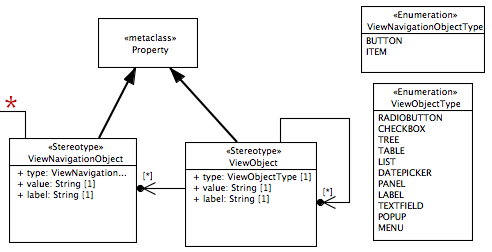
\includegraphics[width=\textwidth]{./img/ProfilProp.png}
\caption{Darstellung der Properties und Enumerations im
Profil}\label{Fig:UMLProfilProp}
\end{center}
\end{figure}\\
In dem Profil wurden zwei Stereotypn als Properties definiert (Abbildung \ref{Fig:UMLProfilProp}). Das \textit{ViewObject} und das \textit{ViewNavigationObject}, die die Widgets in GWT repräsentieren. Durch die Frontendbetrachtung gibt es nur Elemente, die entweder zum Anzeigen von Informationen (\textit{ViewObject}) oder zum Navigieren auf andere Views (\textit{ViewNavigationObject}) dienen. Die \textit{ViewNavigationObject}s können auch für andere Verhaltensspezifikation dienen, die aber im Rahmen dieses Projektes nicht umgesetzt wurden. Die Trennung dieser ähnlichen Elemente musste erfolgen, da es nur so möglich wurde, dass zwar \textit{ViewObjects} andere \textit{ViewObjects} oder \textit{ViewNavigationObjects} enthalten können, bei \textit{ViewNavigationObjects} dies wiederum aber nicht möglich sein sollte. Denn diese beschreiben, mit Button und Item, schon die einfachsten Interaktionselemte.
Den Typ der Property wurde, wie bereits im Konzeptionsteil erläuert (vgl. Abschnitt \ref{AufBProfil}), mit Hilfe von Enumerations festgelegt. Zudem ermöglichen diese eine Reduzierung der unterschiedlichen Modellelemente und gewährleisten so eine bessere Übersichtlichkeit. Im Unterschied zur Konzeption wurde festgelegt, dass Multi-Navigationselemente (wie Table, List, Menu oder Tree) als \textit{ViewObject} definiert sind, die dann wiederum \textit{ViewNavigationObject}s vom Typ \texttt{ITEM} oder \texttt{BUTTON} besitzen können. Die Gruppierung als Items, die zuvor in der Konzeption als \texttt{MENUITEM} oder \texttt{TREEITEM} aufgeführt wurden (vgl. Abschnitt \ref{AufBProfil}), ermöglichte es, die Generierung einfacher zu gestalten. Denn alle Items können nun gleich generiert werden, unabhängig davon, welchem \textit{ViewObject} sie angehören. Zusätzlich können \texttt{TREEs}, \texttt{LISTs} sowie \texttt{TABLEs} auch einfache Widgets wie beispielsweise Textfelder enthalten. Somit müssen diese also keine Interaktionselemente beinhalten, wodurch diese Trennung durch \texttt{ITEM} und \texttt{BUTTON} erforderlich wurde.

Bei den Widgets lag der Fokus auf den jeweils wichtigsten Elemente (\texttt{BUTTON}, \texttt{ITEM}, \texttt{TEXTFIELD}, \texttt{TABLE} etc.), die im späteren Verlauf des Projektes auch alle generierbar sein sollten. Diese lassen sich in zukünftigen Versionen einfach erweitern, indem man zusätzliche EnumerationLiterals hinzufügt und die Erstellung dieser im Generator anpasst. Die weiteren Attribute wie \texttt{value} oder \texttt{label} wurden dann in dem entsprechenden Stereotyp als Attribut hinterlegt.
Hierbei ist anzumerken, dass das \textit{ViewNavigationObject} in der ersten Fassung noch ein zusätzliches Attribut \texttt{goToView} besaß. Im Verlauf der Implementierung des Generators, stellte sich das als fehlerhaft heraus, da dies eine 1:1 Beziehung beschrieb und eine View nur von einem einzigen \textit{ViewNavigationObject} angesteuert werden konnte. Um dieses Problem zu beheben, wurde eine Assoziation im Profil hinzugefügt. So ist es jetzt beispielsweise möglich, dass unterschiedliche Impressum-Buttons auf die gleiche \textit{ViewImpl} 'Impressum' verweisen können. \\
\begin{figure}[ht]
\begin{center}
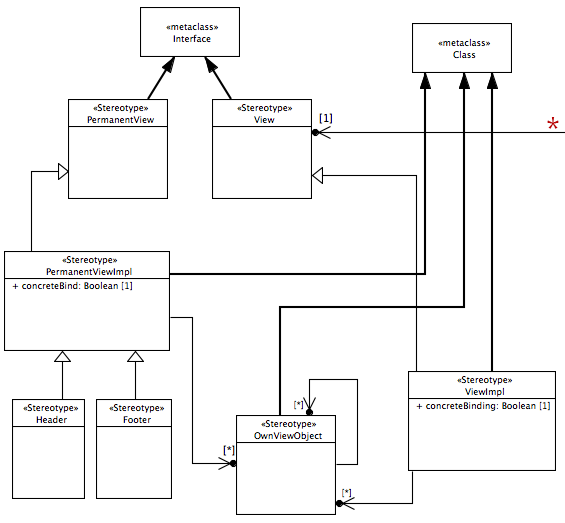
\includegraphics[width=\textwidth]{./img/ProfilClass.png}
\caption{Darstellung der Classes und Interfaces im Profil}\label{Fig:UMLProfilClass}
\end{center}
\end{figure}

Es wurden die Stereotypn \textit{View} und eine \textit{PermanentView} von der Metaklasse Interface abgeleitet. Diese bieten hilfreiche Schnittstellen für deren Implementierungen. Die beiden Interfaces werden als Stereotyp \textit{ViewImpl} und \textit{PermanentViewImpl} der Meta Klasse class implementiert (Abbildung \ref{Fig:UMLProfilClass}). Durch Erstellen des Boolean Attributs \texttt{concreteBinding}(in der Konzeption \ref{AufBGenerator} noch binding genannt),  ist es z.B. möglich, den entsprechenden \texttt{bind}-Befehl über den Generator zu setzen. Der Defaultwert des Attributs ist \texttt{true}, da im Regelfall kein Interface existiert oder es wenigstens eine Implementierung von einem speziellen Interface gibt. In diesem Fall gibt es immer nur diese eine View Implementierung, die angezeigt werden kann. Sollte es aber mehrere Implementierungen zu einem Interface geben, muss das \texttt{concreteBinding} dieser auf \texttt{false} gesetzt werden. Dadurch wird dieses im Anwendungsfall entsprechend berücksichtig und gleichzeitig nur die richtige View ausgewählt.
Anfangs gab es für die Interfaces mehrere Lösungsansätze. In der ersten Fassung beispielsweise erbten auch \textit{Footer} und \textit{Header} direkt vom \textit{View} Interface. Da \textit{Footer} und \textit{Header} aber eigentlich \textit{PermanentViewImpl} mit vordefinierten, festen Positionen sind, war es sinnvoller diese direkt von der \textit{PermanentViewImpl} erben zu lassen. So wie es letztendlich in der Endfassung auch umgesetzt wurde.\\

Für spezielle Klassen wurde noch der Stereotyp \textit{OwnViewObject} hinzugefügt, der es dem Entwickler später ermöglichen soll, diese zu View Implemntierungen hinzuzufügen. Die \textit{OwnViewObjects} dienen als eigenständige Widgets, die die Möglichkeit bieten andere GWT Widgets zu enthalten. \\

Damit auch hier der Umfang des Arbeitsaufwandes für den GWT Entwickler so gering wie möglich gehalten wird, wurden im Profil die Stereotypn, wie in der Ziel Architektur vorgesehen, Activity und Place nicht angelegt. So müssen sich die Entwickler im M1 Modell zu diesen Klassen keine Gedanken mehr machen, denn mit Hilfe des Generators werden diese automatisch zur entsprechenden View generiert. Auch der direkte Stereotyp Model, welcher beispielsweise die Schnittstelle zu einer Datenbank repräsentiert hätte, entfällt in dem Profil. Denn im Projekt war diese Backend-Anbindung nicht vorgesehen.